\section{Introduction}

With an unprecedented engagement of the scientific community at large, the Vera C. Rubin Observatory (hereafter Rubin) has designed a process of incremental improvements to the survey strategy to maximize the overall scientific throughput of the Legacy Survey of Space and Time (LSST). The high-level requirements for the LSST are set by four science pillars: probing dark energy and dark matter, building an unprecedented inventory of the Solar System, mapping the Milky Way and Local Volume, and exploring the transient universe. 

These requirements are described in \cite{LPM-17} ---hereafter the Science Requirements Document, or \citetalias{LPM-17}---, but significant flexibility remains in survey cadence within these requirements. The optimization of the survey strategy process is aimed at maximizing science for the four science pillars and increasing the portfolio of LSST science by tuning the survey strategy and cadence within the SRD requirements (\citetalias{LPM-17}).

As part of this process, the Survey Cadence Optimization Committee (SCOC) was set up by Rubin's Science Advisory Committee in 2018 to solicit, review, and integrate community feedback and make recommendations for the implementation of the LSST survey strategy to the Director of Operations. This document constitutes the third SCOC recommendation, resulting from the Phase 3 process of survey design which started in January 2023, after the delivery of the Phase 2 recommendation  (\citealt{PSTN-055} ---hereafter \citetalias{PSTN-055}--- and the baseline simulation \texttt{baseline\_v3.0}. \cite{PSTN-056} (this document) is planned to be the last recommendation for the LSST as a whole before the start of LSST. However, the SCOC will refine the plan for Y1 in particular and the LSST in general in light of commissioning outcomes; reviews of the survey strategy will continue throughout the 10-year survey,  renewing its recommendation on an annual basis (\autoref{sec:next}). 

The Phase 3 recommendation (this document) responds directly to the questions left open in Phase 2 (\citetalias{PSTN-055}) and updates and refines previous recommendations (\citetalias{PSTN-055} and  \citetalias{PSTN-053}) The present document generally does not reiterate previous recommendations that have not changed.




The document is structured as follows.
%The open questions identified in \citetalias{PSTN-055} Section 4  are included here for the reader's convenience in \autoref{sec:openquestions}. The SCOC recommendations relative to those questions follow each question. 
Each of the points left for deliberation in  \citetalias{PSTN-055} is discussed in \autoref{sec:openquestions}. 
Additional changes to the survey strategy are described in \autoref{sec:additional} and changes to the simulations, beyond the content of this recommendation, in \autoref{sec:opsimchanges}. 
The current recommendation is summarized in \autoref{sec:summary} and the \baseline{4.0} simulations are described in \autoref{sec:baseline4_0}.
The planned activities of the SCOC in Operations, and topics that the SCOC should focus on in the next round of deliberations, including the process of interaction with the community and iterative optimization of the LSST during Operations follow in \autoref{sec:next}.
This document includes definitions of acronyms and terms used in \autoref{sec:acronyms}.

The simulations discussed in this recommendation are available at \url{https://usdf-maf.slac.stanford.edu}

In the spirit of reproducibility, a notebook that generates the figures contained in this notebook is available at \url{https://github.com/lsst-pst/pstn-056/blob/main/notebooks/pstn-056-figures.ipynb}.

\clearpage
%In \autoref{sec:process} we describe .

\section{Executive Summary of the Phase 3 recommendation}


To help the reader parse the content that follows, we note that the LSST survey is actually an ensemble of surveys. It includes a main survey, known as Wide Fast Deep (WFD), which by SRD ``goal'' (minimum) requirement should receive more than 825 (750) observations and cover at least 18,000 (16,000) square degrees, and a Galactic Plane (and Bulge) survey. Furthermore, a WFD low-dust region is defined with limits $-70^o \leq \mathrm{Dec} \leq +12.5^o$ for 
$\mathrm{RA} \sim   7-18 h$ and $-72^o \leq \mathrm{Dec}\leq +3^o$
for $0 \lesssim \mathrm{RA} \lesssim 7$ h and $18 h \lesssim \mathrm{RA} \lesssim 24 h$, with the addition of the Virgo cluster, as of \citetalias{PSTN-055}.  Special regions in the LSST include the LMC, SMC, South Celestial Pole (SCP), and North Ecliptic Spur (NES). Microsurveys, or surveys performed with a different cadence from the WFD and that require $<3\%$ of the LSST time can be performed and \citetalias{PSTN-055} committed to a twilight Near-Earth-Objects (NEO) microsurvey in the first year of LSST, Y1, and to accept further proposals for future microsurveys after the start of LSST. A Target of Opportunity program was recommended for up to $3\%$ of LSST time in \citetalias{PSTN-055}.

Notable updates from previous recommendations, and corresponding changes to the baseline, include updating system throughputs,  expectations for engineering time (particularly in Y1), and slew performance; tweaking the filter balance in response to throughput changes; refining observing choices in the Galactic Plane, Bulge, and LMC/SMC/SCP; defining the implementation plan for the ToO program; recommending single visit exposures over visits implemented in ``snaps''; investigating new rolling strategy options; refining the DDF observing plans.


\subsection{Note on how to read the SCOC plots}

The SCOC typically reviews the outcome of metrics measuring system performance and science outcomes built within the Metric Analysis Framework \citep{2014SPIE.9149E..0BJ}, hereafter MAFs. MAFs are reviewed across multiple simulations of the 10-year sequence of LSST observations, each simulation referred to as an \opsim\, to compare scientific performance. In this document, you will see sky maps measuring quantities by healpixels (\eg, number of visits, or any MAF). The typical sky pixelization that underlies the metric calculations the SCOC reviews is 128 sides healpixels (covering an area $\sim 0.2\mathrm{deg}^2$), although for particularly computationally intense MAFs this can be turned down to 64 or 32. You will see metric plots in the following styles: 



{\bf Heatmaps}: \autoref{fig:heatmap} -
the divergent color scheme shows improvements in metrics in blue and drops in performance in red. Note that different heat maps may show different ranges in the color scheme, but the SCOC typically considers changes of more than a few percent to be significant and less than a few percent to be in the noise. One of the \opsim s is chosen as a reference and the corresponding column will look neutral in color.

\begin{figure}
  \centering
    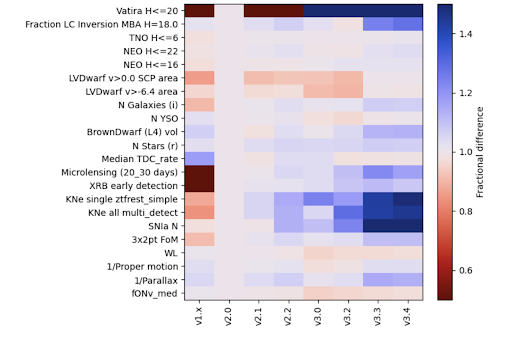
\includegraphics[width=0.95\textwidth]{figures/v1-v34heatmap.png}
\caption{A heatmap produced by the Observing Strategy team for the SCOC. The plot compares the performance of selected metrics across baseline simulations from \baseline{1.X} (original survey strategy) through \baseline{3.4}. In these plots, an \opsim\ is selected as the reference and the performances of all other \opsim s are shown relative to that. That is: the reference \opsim\ (\baseline{2.0} in this case) has MAF=1 for all the metrics. Blue colors indicate a positive metric value, \ie\ an improvement. Red colors indicate a performance drop with respect to the reference \opsim. Significant changes in the observing strategy can be seen to impact nearly all metrics (the whole column). For example: the changes between \baseline{3.2} and \baseline{3.3} are due to the updated filter throughput models corresponding to updated plans for mirror coating (discussed in \autoref{sec:filterbalance}). These changes lead to an overall increase in survey depth, resulting in all tracked metrics having the same or better performance (bluer or the same color as the previous column).}
\label{fig:heatmap}
\end{figure}


\FloatBarrier

{\bf Radar plots}: \autoref{fig:radar} - when comparing small numbers of metrics and few \opsim\ we often use radar plots. Each corner of the radar plot corresponds to a metric, and the colored lines inside the plots that join each corner show metric performance. In these plots, the reference \opsim s looks like a N-gone (or N-sided circle). Where the MAF performance shows improvements compared to the reference \opsim\ the point lies outside of the N-gone, where there is a loss, it sits inside. The range of performance changes, so readers should carefully inspect the plot to see the performance scaling going in and out of the N-gone (typical values are 0.9-1.1). 

\begin{figure}
  \centering
    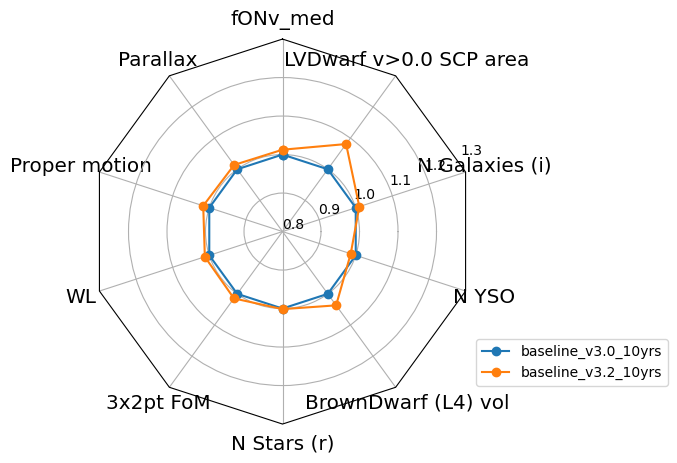
\includegraphics[width=0.95\textwidth]{figures/radarplot.png}

\caption{A radar plot comparing the performance of MAFs under different filter swapping schemes (see \autoref{sec:filterswap}). This plot compares \baseline{3.0} with \baseline{3.2}. All metrics shown perform as well or better in \baseline{3.2} as shown by the orange points laying outside of the blue polygon, except for \texttt{N~YSO}. However, the loss in \texttt{N~YSO} is minimal and not statistically significant. The range of the axis is 0.8 to 1.3, indicating that a point lying in the center would measure a performance 20\% worse than the reference \opsim, and a point on the outer perimeter would indicate a 30\% improvement.}
\label{fig:radar}
\end{figure}


\FloatBarrier

%{\bf Line plots}: \autoref{fig:lineplot} -
%line plots can show multiple \opsim s and metrics at once. The comparison metric will sit as a horizontal line at 1.0 throughout the plot. The regions outside of the 3\% range we typically consider not-significant are shaded in red (for MAF loss) and green (for MAF gains).


%\begin{figure}
%    \centering
%    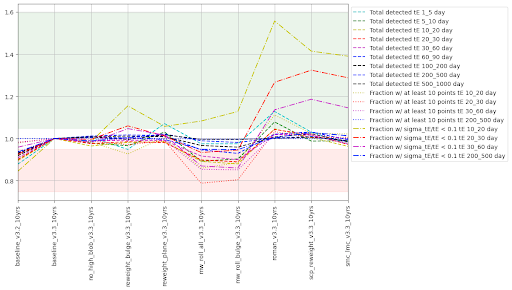
\includegraphics[width=0.8\linewidth]{figures/lineplot.png}
%    \caption{Line plot showing the performance of a collection of \opsim\ designed for the Milky Way Task Force (see \autoref{sec:galaxy}) and the corresponding performance for a collection of related Microlensing MAFs. The comparison \opsim\ is \baseline{3.3} (where all the MAFs meet at $y=1$.)}
%\label{fig:lineplot}
%\end{figure}
%\FloatBarrier
